%%%%%%%%%%%%%%%%%%%%%%%%%%%%%%%%%%%%%%%%%%%%%%%%%%%%%%%%%%%%%%%%%%%
%                                                                 %
%                            CHAPTER THREE                        %
%                                                                 %
%%%%%%%%%%%%%%%%%%%%%%%%%%%%%%%%%%%%%%%%%%%%%%%%%%%%%%%%%%%%%%%%%%%

\chapter{CAVITY-BASED CONFORMAL MESH ADAPTATION}
\label{chap:adapt}

\section{In Context}

The mesh adaptation methods in this work are
conformal, general, and cavity-based.
In the following Sections we define these
terms in contrast to other techniques for
modifying meshes.

\subsection {Conformal and General}

They are conformal in the sense that the boundaries of all
elements (Section \ref{sec:def_complex}) are composed
of the set of entities expected by that element's
topological template (Section \ref{sec:topo_template}).
In other words, we avoid the ``hanging node" scenarios
introduced by non-conformal mesh modification techniques.
Typically, non-conformal mesh modification also restricts
itself to subdividing input elements into more elements,
or undoing such subdivisions which were done before.
Figure \ref{fig:hex_amr} illustrates such a method,
and clearly shows the hanging nodes introduced.

\begin{figure}
\begin{center}
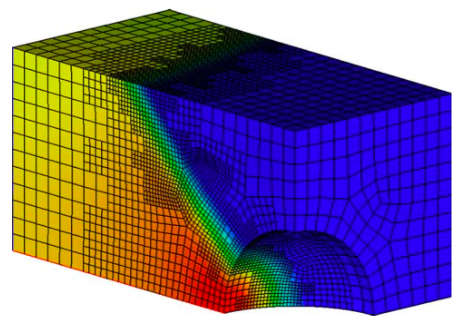
\includegraphics[width=0.6\textwidth]{hex_amr.png}
\caption{Non-conforming parent-child adaptive mesh refinement
\cite{kirk2006libmesh}}
\label{fig:hex_amr}
\end{center}
\end{figure}

Non-conforming meshes require additional support from
the PDE-solving code to deal with hanging nodes, and typically
no more than one level of refinement is allowed between adjacent
elements.
The more important limitation is due to non-conforming methods
typically being parent-child methods, which fundamentally limits
them to the topology (and geometry) of the coarse input mesh.
If this input mesh is more fine than necessary in some areas,
it cannot be coarsened.
If moving objects or object deformation cause input elements
to become highly compressed or even inverted, parent-child
refinement can never correct or prevent this.
New node placement when refining along a curved boundaries poses
a similar issue to that of physical deformation.
For these reasons we take a general approach, employing
local cavity-based mesh modification operations which are
able to coarsen beyond the input mesh and correct low-quality
elements in the input mesh.

\subsection{Cavity-Based}
\label{sec:cavity}

We restrict ourselves to local cavity operations,
meaning that the transformation from input to output meshes
can be expressed as a series of cavity modifications, each
of which can in turn be expressed as the removal of
a small number of mesh entities followed by the addition
of a small number of mesh entities.

In general, a cavity can be defined as a manifold sub-domain
of the mesh defined by a set of elements from the original
input mesh.
A cavity undergoes a modification, which changes the discretization
(set of mesh entities) of its interior but leaves its ``boundary" unchanged.
In order to allow changing the discretization of the overall
mesh boundary (i.e. the geometric model boundary)
we use a relaxed definition of a cavity boundary
(shown in Figure \ref{fig:cavity_boundary}) which only includes
entities that are also adjacent to elements outside the cavity.
This is the minimum requirement for the method to be conformal:
it must preserve the topology of this relaxed boundary.
For efficient parallel execution, we also require that attributes
of those boundary entities also remain unchanged.
This includes geometric classification, as discussed in Section
\ref{sec:ma_coarsen} and illustrated in Figure \ref{fig:surf_collapse}.
This allows two cavities to be modified simultaneously by two
threads or processes, so long as the cavities do not overlap
(i.e. they do not share elements).
They may be adjacent (share a subset of their boundaries) and
need not coordinate because nothing about the shared boundary
will be changed by either one.

\begin{figure}
\begin{center}
\includegraphics[width=0.6\textwidth]{cavity_boundary.png}
\caption{Relaxed definition of cavity boundary excludes geometric boundary}
\label{fig:cavity_boundary}
\end{center}
\end{figure}

Some benefits of using local cavity operations are:
\begin{enumerate}
\item It allows more straightforward and reliable parallelization of
mesh adaptation (see Section \ref{sec:cavity_sched}).
\item It allows much more careful control of the effects that mesh
adaptation has on the simulation fields attached to the mesh.
\end{enumerate}

On the other hand, the set of known cavity operations
have been found by the trial and error of researchers,
and there are many properties which they are not guaranteed to
achieve.
The most successful set of cavity operators are those
which operate on simplex meshes, due ultimately to the
fact that a simplex is the simplest polytope of a given dimension
and that, conversely, more complex polytopes provide fewer
valid configurations.
In our work, we separate cavity operators into several categories:
\begin{enumerate}
\item Refinement: create a strictly more detailed discretization
than the input. Guaranteed not to invert elements, but not to
preserve any element quality. Guaranteed to exactly preserve
the distribution of fields.
\item Coarsening: create a strictly less detailed discretization
than the input. No guarantees it can be done without reducing
or negating quality, so it must be checked.
By definition, cannot exactly preserve the distribution of the fields.
\item Shape correction: typically maintains similar level of detail,
modifies connectivity to improve minimum element quality.
There is no known method guaranteed to raise all elements to a quality
that is useful for simulation and adaptation, but heuristic
methods can achieve great results in practice \cite{klingner2008aggressive}.
\item Snapping: procedures intended to improve the discrete
mesh approximation of a continuous curved boundary.
\end{enumerate}

\section{Related Work}

There have been several iterations of the MeshAdapt
library developed at RPI.
One of the earliest publications by De Cougny and Shephard
\cite{de1999parallel} outlines the three basic steps and goes into some detail
on a use of independent sets for coarsening purposes
(an idea that we extend significantly in Section \ref{sec:indset}).
Later, substantial extensions were introduced by Li on anisotropy using the metric
tensor and the selection of operators for shape correction
\cite{li20053d,li2003mesh}.
Our implementations of tetrahedral edge swaps make use
of guidance on fast implementation by Olivier-Gooch \cite{freitag1997tetrahedral}.
Researchers at INRIA have provided useful mathematical foundations
for handling the anisotropic metric tensor field
\cite{frey2005,alauzet2006parallel,loseille2015parallel},
and work at the Catholic University of Louvain explored
the use of mesh adaptation to respond to moving objects
\cite{compere2010mesh}, a path we continue with our Omega\_h work.

\section{MeshAdapt Methods}
\label{sec:ma_methods}

\subsection{Template Refinement}
\label{sec:ma_refine}

The MeshAdapt library uses edge-based refinement templates for its refinement step.
The way these work is that all edges whose metric length exceeds some threshold
$l_{\text{up}} > 1$ are marked for refinement.
Then each element takes into account the subset of its edges which are marked
for refinement, and chooses one of many possible subdivision patterns
(refinement templates) based on this subset of edges.
Figure \ref{fig:tet_templates} illustrates these templates in the case of tetrahedra.
In fact, the center template shown for three marked edges has two variants which
are symmetric by reflection but not by rotation.
In total, this means there are 12 rotationally unique tetrahedron refinement templates.

\begin{figure}
\begin{center}
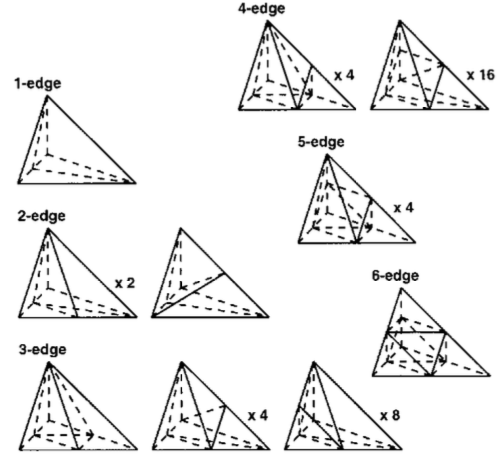
\includegraphics[width=0.6\textwidth]{tet_templates.png}
\caption{Tetrahedral refinement templates}
\label{fig:tet_templates}
\end{center}
\end{figure}

One benefit of the use of refinement templates is that adjacent elements can be refined
simultaneously, so all edges, faces, and regions of the mesh can be modified in
a nearly embarrassingly parallel fashion once the set of marked edges is identified.
Another benefit is that the gradation of the mesh is more explicitly controlled
compared to methods which split edges independently.
However, refinement templates have some drawbacks as well:
\begin{enumerate}
\item In some cases, a subset of the template is a polyhedron that cannot be
subdivided into tetrahedra without introducing an extra vertex within the
parent tetrahedron.
In particular, Sch{\"o}nhardt's polyhedron can appear (see Figure
\ref{fig:schonhardt}).
This reduces the predictability of refinement and makes it more difficult
to transfer solution.
\item Other cases introduce a geometric decision, such as the case
when all edges of a tetrahedron are refined, or even when two edges
of a triangle are refined. This also reduces predictability.
\item It takes substantial code to implement all rotationally unique
combinations for all the relevant element polytopes.
This increases the likelihood of errors and decreases the productivity
of modifying any aspect of refinement.
\item Due to the simultaneous nature of the operation and the difficulty
of predicting the outcome, it is prohibitively difficult to reject
a local portion of the refinement based on criteria such as new elements
having too low quality.
\end{enumerate}

\begin{figure}
\begin{center}
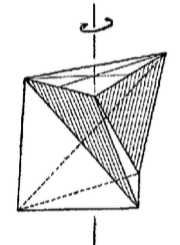
\includegraphics[width=0.2\textwidth]{schonhardt.png}
\caption{Sch{\"o}nhardt's irreducible polyhedron
\cite{Schonhardt1928}}
\label{fig:schonhardt}
\end{center}
\end{figure}

\subsection{Coarsening}
\label{sec:ma_coarsen}

Like other adaptation libraries, MeshAdapt implements
coarsening via edge collapses.
Figure \ref{fig:collapse} shows a typical edge collapse
in a tetrahedral mesh for reference.
One vertex in the mesh is ``moved" onto another vertex which is adjacent
via a mesh edge, collapsing this edge and all its adjacent
faces and regions.
For programming purposes, when dealing with sets of entities we
can call those being removed the ``collapsing" set and those being
conceptually elongated to fill the cavity as the set to ``keep".
In practice all old entities are removed and the set of entities to keep
is rebuilt with modified connectivity (where they were adjacent to the
collapsed vertex, now they are adjacent to the kept vertex).

\begin{figure}
\begin{center}
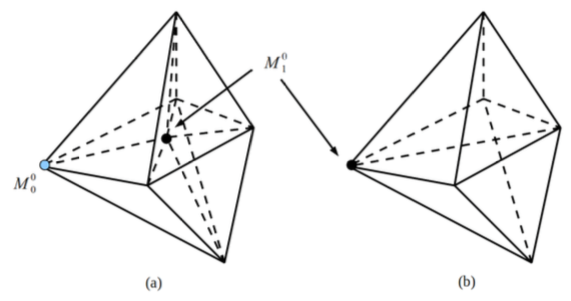
\includegraphics[width=0.6\textwidth]{collapse.png}
\caption{Edge collapse in tetrahedral mesh
\cite{lu2011developments}}
\label{fig:collapse}
\end{center}
\end{figure}

Edge collapsing is an operation which, if not properly controlled,
can invalidate the mesh topologically or undo its topological similarity
to a CAD model \cite{schroeder1990combined}.
MeshAdapt uses a set of checks which is somewhat expensive to compute
but is topologically robust:

\begin{enumerate}
\item The vertex being collapsed must have the same classification as
the edge being collapsed. This preserves similarity to the CAD model by
preventing collapses from the boundary into the interior.
\item If there exists a ring of three edges including the collapsing edge
(Figure \ref{fig:edge_ring}),
then those three edges must bound a single triangle in the mesh.
This prevents collapsing an empty hole in the mesh to zero volume as in
Figure \ref{fig:circle_hole}.
While some \cite{beall1997general} consider Figure \ref{fig:circle_hole}
a valid operation, current mesh data structures assume an entity is uniquely
defined by its set of bounding entities, which precludes the two overlapping
mesh edges that Figure \ref{fig:circle_hole} produces.
In addition, the non-collapsing edge adjacent to the collapsing vertex must have the same
classification as the triangle.
This prevents collapsing a cavity on a curved boundary down to zero volume
(see Figure \ref{fig:surf_collapse}), which would require re-classifying
entities on the cavity boundary (which breaks parallelism guarantees), and
creates no elements in the new cavity (which is problematic for solution transfer).
\item Analogous to the edge ring check, in 3D we check for two triangles which
share a non-collapsing edge and whose remaining two vertices are the endpoints
of the collapsing edge (a ``face ring").
The two triangles and the collapsing edge must bound a single tetrahedron,
and the triangle adjacent to the collapsing vertex must have the same classification
as this tetrahedron.
\item All the resulting tetrahedra must have positive volume.
In the 2D planar case, triangle normals should all be positive in the Z axis.
For straight-sided simplices in an equal-dimensional space (i.e. triangles in 2D
and tetrahedra in 3D), this check on its own can prevent some topological invalidities,
except those in Figure \ref{fig:circle_hole} and Figure \ref{fig:surf_collapse}.
\end{enumerate}

The edge and face ring conditions are more complete versions of those described
by Garimella \cite{garimella1999anisotropic}.
Most of the expense of checking these conditions is in the search procedure
to identify edge rings and face rings, as the naive approach costs $O(n^2)$
comparisons where $n$ is the number of edges (or faces) adjacent to one vertex.
For typical tetrahedral meshes there may be 36 or more faces adjacent to a vertex,
meaning close to 1000 comparisons would be needed.
We can reduce the cost by using a set structure to store the $n$ vertices (or edges)
that may complete a ring from one endpoint, and use its $O(\log(n))$ membership check
capability to reduce the comparison cost to $O(n\log(n))$.

\begin{figure}
\begin{center}
\includegraphics[width=0.5\textwidth]{edge_ring.png}
\caption{Edge ring condition check during edge collapse}
\label{fig:edge_ring}
\end{center}
\end{figure}

\begin{figure}
\begin{center}
\includegraphics[width=0.4\textwidth]{circle_hole.png}
\caption{Illegal collapse of a CAD hole represented by a periodic boundary}
\label{fig:circle_hole}
\end{center}
\end{figure}

\begin{figure}
\begin{center}
\includegraphics[width=0.2\textwidth]{surf_collapse.png}
\caption{Illegal collapse with no new elements and re-classification}
\label{fig:surf_collapse}
\end{center}
\end{figure}

Finally, when applying a series of edge collapses to a mesh, one
must additionally filter the set of edges targeted for collapse
until it forms an independent set, in order to avoid a pathological
sequence of edge collapses reducing large portions of the mesh
down to a single edge.
We resolve this by visiting vertices which are marked for collapse
and unmarking them so long as each edge that needs collapsing
still keeps one adjacent marked vertex.
Similar methods of establishing an independent set were
in use in early versions of MeshAdapt \cite{de1999parallel}
and continue to be used by other adaptation codes
\cite{michal2012anisotropic}.

\subsection{Shape Correction}
\label{sec:ma_shape}

Shape correction, otherwise known in the literature as ``sliver removal",
is one of the most important open problems in tetrahedral meshing.
When meshing a planar domain with triangles, techniques such as
Delaunay refinement can guarantee triangles of a certain quality,
where quality can be measured by angles at corners or the
mean ratio (see Appendix \ref{app:vert_up_deg} for the relationship
between these measures).
However, when meshing a volumetric domain with tetrahedra, there
are no known methods to provably guarantee element quality (dihedral angles
or the mean ratio).
What is typically done is to carry out a method which satisfies
edge length criteria and at a minimum produces positive-volume
tetrahedra.
Following this, heuristic methods (sliver removal) are carried out
to attempt to remove tetrahedra with quality below a constant user-defined
threshold.

Despite these methods being heuristic, their combination can often
give very good results in practice.
The most aggressive approaches
\cite{klingner2008aggressive,dassi2016tetrahedral}
can usually bring tetrahedral dihedral angles into
the range $[30^\circ,130^\circ]$, which is sufficient for
most simulation purposes.
However, these aggressive approaches may be either too expensive
for use in mesh adaptation (which is executed within a
performance-critical simulation), or they may modify the mesh
too much (a large movement of all the nodes in the mesh would
change the physical distribution of the fields defined by values
at the nodes).

Mesh adaptation has the advantage of being provided with an input
mesh, and therefore one can in theory reject any operation which
would decrease the quality of the mesh lower than it was on input.
In this sense, mesh adaptation can guarantee quality at least as good
as the input.
We will see this approach taken to some degree in the Omega\_h methods
described in Section \ref{sec:omega_h-adapt}.
The danger of rejecting operations based on quality is that
if too many operations are rejected then edge lengths will
not conform well enough to the metric field.
However, we are having increasing success with
careful rejection of operations and some researchers
are able to avoid using sliver removal techniques
altogether if their quality requirements are low
enough \cite{loseille20093d,michal2012anisotropic}.

Typically, mesh adaptation libraries implement a balance
between prevention of quality degradation and repairing
quality that has been degraded.
The repair process uses a subset of the known sliver removal
techniques, with a focus on being able to repair the average
sliver using minimal computational resources, while resorting
to more expensive techniques when the cheaper ones fail.

Li describes a fairly comprehensive set of sliver removal
heuristics implemented in an earlier version of MeshAdapt
\cite{li2003mesh}.
The current version uses a similar approach, based on a
taxonomy of sliver tetrahedra.
The taxonomy can be described in terms of some boundary
entity being too close to another boundary entity
of the tetrahedron:
\begin{enumerate}
\item In the first case, we have two vertices being too
close, which is really just an edge being too short.
If quality is low in metric space, this is a case
of an edge which should have collapsed but didn't.
We attempt to more aggressively collapse it by trying
to collapse each edge adjacent to either endpoint vertex.
\item In the second case, we have a vertex being too close
to its opposing triangle face.
Here we try to execute an edge swap (see Figure \ref{fig:swap})
on each of the three edges bounding the opposing triangle face.
(The work of Li suggests that a face split and collapse operation
should also be implemented as future work).
\item In the third case, we have the classic sliver tetrahedron
which has two opposing edges being too close to one another.
We first attempt to perform an edge swap on each of the two
opposing edges.
If that fails, we attempt a double split collapse operation
as shown in Figure \ref{fig:compound}.
\end{enumerate}
Each of the above attempted operations is judged in terms of quality.
If the minimum quality of any element in the cavity after a modification
exceeds minimum quality of any element in the cavity before the
modification, then we say the quality has locally improved.
In most cases, one of the above attempts succeeds.
However, it is possible in practice for none to succeed, in which
case MeshAdapt will leave the sliver as-is.

\begin{figure}
\begin{center}
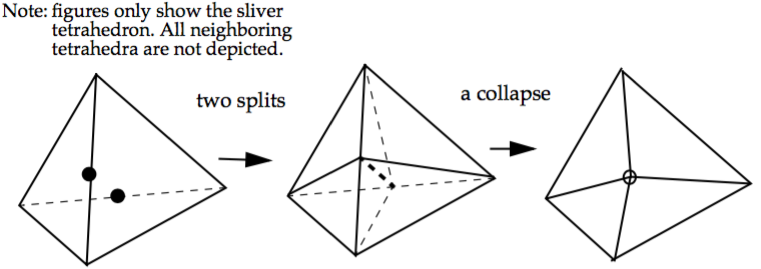
\includegraphics[width=0.8\textwidth]{split_collapse.png}
\caption{Double-split + collapse compound operator
\cite{li2003mesh}}
\label{fig:compound}
\end{center}
\end{figure}

\subsubsection{Edge Swap}
\label{sec:swap}

\begin{figure}
\begin{center}
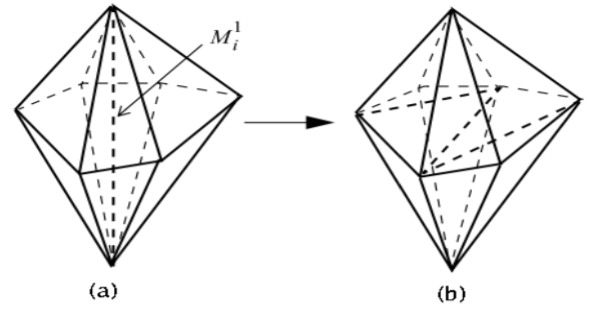
\includegraphics[width=0.5\textwidth]{swap.png}
\caption{Edge swap in tetrahedral mesh
\cite{lu2011developments}}
\label{fig:swap}
\end{center}
\end{figure}

The edge swap operation deserves a detailed consideration due
to its complexity.
Its goal is to remove the elements adjacent to an edge and
replace them with a new set of elements such that the edge
is not recreated.
In the tetrahedral case, this essentially reduces to the problem
of forming an output triangular mesh based on the ``ring" vertices
(those vertices which are opposite to the central edge across
an input triangle), as Figure \ref{fig:swap} illustrates.
Furthermore, since this operation is used almost exclusively
for the purpose of repairing quality degradation (sliver removal),
what we are interested in is finding the triangular mesh of the
ring such that the resulting tetrahedral mesh of the cavity
contains elements above a certain quality.
The quality to beat is usually the lowest quality input
tetrahedron, i.e. we want to at least improve the minimum quality.

A naive search of the space of possible triangular meshes
can be quite expensive, so we use an optimized algorithm
described by Freitag and Ollivier-Gooch \cite{freitag1997tetrahedral}.
The algorithm consists of limiting oneself to rings of a
certain number of vertices (in our case, not attempting
rings that have more than 7 vertices), and storing integer
tables describing all possible trianglulations of such rings.
The triangulations are described in terms of unique triangles
(two triangulations may share the same triangle).
Because the qualities of the two adjacent tetrahedra adjacent
to such a triangle are uniquely defined, then if either quality
is below the target threshold, all triangulations that include
that triangle can be ignored.
Otherwise, the lower of the two qualities is stored in association
with the unique triangle, to avoid later re-computation.

\subsection{Overall Steps}

Listing \ref{lst:ma} shows an abbreviated version of the C++
code for MeshAdapt's main function.
The central loop executes a fixed number of iterations.
At each iteration, we first coarsen as described
in Section \ref{sec:ma_coarsen}, followed by refinement
as described in Section \ref{sec:ma_refine}.
We perform coarsening before refinement because this
should reduce the peak memory usage between the two
operations.
Shape correction is performed after the main loop
has completed, using the algorithm in Section \ref{sec:ma_shape}.
The functions whose names end in \texttt{Balance} execute
parallel load balancing.
We treat mesh elements as the units being balanced,
and assign weights to them based on the metric space
volume defined by Equation \ref{eq:metric_volume}.
Either graph partitioners \cite{devine2002zoltan} or
diffusive partitioning methods \cite{SmithParma2015}
may be used at each step.

\begin{lstlisting}[float,style=dan-style,caption=MeshAdapt main function,label=lst:ma]
void adapt(Input* in) {
  Adapt* a = new Adapt(in);
  preBalance(a);
  for (int i = 0; i < in->maximumIterations; ++i) {
    coarsen(a);
    midBalance(a);
    refine(a);
  }
  fixElementShapes(a);
  postBalance(a);
  delete a;
  delete in;
}
\end{lstlisting}

\section{Omega\_h Methods}
\label{sec:omega_h-adapt}

The Omega\_h code aims to provide MeshAdapt-like functionality
on a wide variety of computing hardware.
Due to the restrictions introduced by shared memory parallelism,
Omega\_h initially chose a simpler set of algorithms to reduce the
cost of redesigning each algorithm for portability.

There are several key characteristics of MeshAdapt's design
which need to be changed in order to execute efficiently with
high degrees of shared memory parallelism (e.g. on GPUs):
\begin{enumerate}
\item The assumption of a persistent thread which can maintain
substantial amounts of local data (e.g. a data structure
representing a mesh partition) and act on that data in serial
is invalid for GPUs, because the increased degree of parallelism
requires lowering the per-thread overhead in memory use and runtime.
Shared memory parallelism is better expressed at the loop level
(see Section \ref{sec:openmp}), and per-thread data should be avoided.
This means data storage concerns (data structures) move up to
the process level (in terms of software) and up to the
node level (in terms of hardware).
\item Modification of the mesh cannot be based on a local \emph{series}
of single entity additions and removals that are immediately
applied to the mesh, because this
introduces increasing contention on the mesh data structure
as the number of threads increase.
Most other research in shared-memory parallelization of mesh modification
has focused either on methods which assume the degree of parallelism
is somewhat small \cite{remacle2015two} (as it is in CPUs) or
methods which use entity-level non-deterministic mutual exclusion
mechanisms \cite{navarro2011parallel}.
We instead propose a deterministic independent set selection system
in Section \ref{sec:indset} that allows us to go from one
simple static structure to another
(the data structure is described in Section \ref{sec:osh_static}).
\item The operations that are performed in parallel should
avoid making use of dynamic local memory allocation
(see Section \ref{sec:cuda}).
For example, when threads need access to variable-length adjacency
data such as upward adjacencies, it is better for them to
cooperate and form a single data structure representing said
information for all entities, instead of having each thread
recompute its portion on demand during a higher-level operation.
\end{enumerate}
Altogether, this results in the need to write the entire program
in an array-based and loop-based style and requires algorithms that
are intuitively expressed in that style.

We have designed such alternative algorithms for performing mesh
adaptation, and so far they have demonstrated
comparable and in some cases higher quality results
for simplex mesh adaptation.
Additional efforts are still underway to examine algorithmic details,
and additional test cases are being developed in collaboration with
other research groups to better qualify mesh adaptation methods,
independent of parallelization.

The following sections describe the algorithms implemented
in Omega\_h in contrast to those of MeshAdapt.

\subsection{Refinement}
\label{sec:osh_refine}

Instead of using template-based refinement, Omega\_h
uses single edge splits, meaning a single edge is
bisected and adjacent elements are bisected
at a single operation.
Unlike the simultaneous execution that is possible
with template-based refinement, only edge
splits whose cavities do not overlap can be
applied simultaneously (see Section \ref{sec:indset}
for how such splits are selected).
Several researchers have similarly had success
using only single edge splits rather than
template-based refinement
\cite{compere2010mesh,loseille20093d,michal2012anisotropic}.
Like MeshAdapt, Omega\_h marks all edges whose
metric length exceeds some threshold (typically $\sqrt{2}$) as candidates
for edge splits.

Omega\_h uses a more accurate formula to measure
edges when determining whether to split or collapse them.
This formula, shown as Equation \ref{eq:metric_length2}
is suggested by Loseille and L{\"o}hner \cite{loseille20093d} and
is based on the assumption that the desired length varies
geometrically along the edge ($h(t)=h_a^{1-t}h_b^t$ where $h_a$ and $h_b$
are the desired lengths at the endpoints).
This assumption is consistent with the Log-Euclidean interpolation method we
use for the metric tensor (see Section \ref{sec:metric_interp}).

\begin{equation} \label{eq:metric_length2}
\tilde{l} =
\frac{\tilde{l}_a - \tilde{l}_b}{\log\left(\tilde{l}_a / \tilde{l}_b\right)}
\quad
\tilde{l}_a = \frac{l}{h_a},\quad
\tilde{l}_b = \frac{l}{h_b}
\end{equation}

Omega\_h then unmarks any edges whose splitting
would produce elements of low mean ratio quality (typically less than $20\%$).
There is a trade-off here between two desired outcomes.
On the one hand, when mesh adaptation is used to control discretization
error, it is preferable to produce meshes of higher than desired resolution
as opposed to lower than desired (in many cases the latter is unacceptable).
Combined with the fact that refinement cannot technically produce
inverted elements or invalid meshes, this is a strong motivation to immediately
and unconditionally refine all edges that exceed a given threshold.
On the other hand, immediate refinement can produce elements of arbitrarily
bad quality, making it increasing difficult to apply future mesh modifications
and driving numerical conditioning of the physical simulation to unwanted extremes.
Since computers use finite precision arithmetic, there are cases in practice
where the refined element volumes are indistinguishable from zero to the computer.
In Omega\_h, we choose to avoid immediate refinement that would violate
quality criteria under the assumption that, in most cases, subsequent
operations (including other edge splits) will improve the situation
sufficiently that the deferred refinement will eventually be accepted
(see the loop in Listing \ref{lst:osh}).
This is especially important when using single edge splits instead of
applying refinement templates, because the order in which edges are split
strongly affects the resulting quality.
We have confirmed that at the end of adaptation we do meet the desired
upper bound on metric edge length in the cases considered to date.

\subsection{Coarsening}
\label{sec:osh_coarsen}

Like MeshAdapt, Omega\_h uses single edge collapses
for mesh coarsening.
Since all operations in Omega\_h use the quality-driven
independent set system described in Section \ref{sec:indset},
that explicitly takes care of the need for an independent
set of collapsing vertices.
Edge collapses have some confusion in what their ``key" entity is,
because in reality it is the combination of an edge and one
of its endpoint vertices that defines a collapse.
We first mark all edges whose metric length is beneath
some threshold (typically $1/\sqrt{2}$) as candidates to collapse
via either endpoint.
In addition, Omega\_h will mark all edges adjacent to either endpoint
of a short edge as additional candidates, since collapsing an endpoint
along one of these additional edges may still elongate it.
Then, for all candidate edges, collapses in the allowed directions are evaluated
using almost all of the checks described in Section \ref{sec:ma_coarsen}.

Omega\_h saves time by skipping the full edge ring and face
ring checks, replacing them with a requirement that each $d$-dimensional simplex
adjacent to the collapsing edge must be classified on the same geometry
as its $(d-1)$-dimensional side adjacent to the collapsing vertex.
In other words, Omega\_h checks for the problematic case shown in Figure
\ref{fig:surf_collapse}, but not for the case in Figure \ref{fig:circle_hole}.
As a result, Omega\_h requires that the input mesh, model or metric be
constructed such that the case in Figure \ref{fig:circle_hole} doesn't arise.
One simple way to ensure this is to mesh ``holes" in the geometry.
For Omega\_h's first target applications,
this makes sense because the interaction of both the fluid and the structure
is of interest.
Barring that solution, one can topologically break up periodic geometry,
for example a periodic CAD edge becomes three or more edges,
which is quite reasonable in the vast majority of cases.

Omega\_h also applies the same quality restriction to coarsening
that it applies to refinement, i.e. changes are not accepted if they produce
elements below a user-defined threshold.

Finally, Omega\_h implements what we call ``overshoot protection"
as suggested by Michal and Krakos \cite{michal2012anisotropic}.
This means that edge collapses are rejected if they would create
new edges that are longer than the edge refinement threshold
from Section \ref{sec:osh_refine}.
This restriction allows us to alternate refinement and coarsening
without entering an infinite loop in which a collapse operation
is exactly undone by a refinement operation, which is then
undone by a subsequent collapse, etc.

We mark candidate collapses using two boolean flags per edge, one for each
endpoint.
Once all collapses that violate the checks mentioned above are unmarked,
we move the focus of the problem from edges to vertices.
To do this, every vertex chooses a single adjacent candidate edge collapse
which is the one it will represent for the remainder of the coarsening operation.
The selection is made first preferring the shortest edge
(as suggested in \cite{michal2012anisotropic}), preferring
higher element qualities if lengths are equal, and ties in
both length and quality are broken using global entity numbers.
All others collapses in which the vertex could have participated for which it is an endpoint are discarded.
Now the independent set selection in Section \ref{sec:indset} is used
with vertices as the keys and their selected collapse qualities as the
values.
The selected independent set of vertices is then collapsed, along each
vertex's chosen edge.

\subsection{Shape Correction}
\label{sec:osh_shape}

Omega\_h uses simpler and yet possibly more effective shape correction logic.
We have found that it is beneficial to consider a wider portion of the
mesh surrounding a sliver when attempting to remove said sliver, rather
than being overly concerned with the particular shape of said sliver.
Omega\_h has a user-defined parameter for how many layers of elements
around a sliver will be considered.
In this case, layers are defined by elements adjacent to one another
across faces, simply because this graph is much cheaper to compute
than that of elements adjacent via vertices.
For every sliver, elements that are at most the specified distance
via face adjacency are marked as being involved in sliver removal.
Then we do one of two things:
\begin{enumerate}
\item Mark all edges of all considered elements as candidates for edge swaps.
For each such edge we compute the best possible edge swap operation
using the optimizations described in Section \ref{sec:swap},
and give those quality values to the method in Section \ref{sec:indset} to
select a set of edge swaps to perform.
Only edge swaps which locally improve the quality in their cavity are accepted.
\item Mark all vertices of all considered elements as candidates for collapsing.
For each of these vertices, we consider collapsing it along any adjacent edge.
This is just a marking process, after which the procedure in Section \ref{sec:osh_coarsen}
is carried out, with the only difference being that for a collapse to be accepted,
the quality in the cavity must locally improve, instead of being above a
constant threshold.
\end{enumerate}
Note that although these algorithms describe using layers around a sliver,
they remain cheap because the layers need only be marked, after which only
small cavities around the marked elements are considered.
The full set of elements marked around a sliver is never collected or examined
as a whole in any way.
The marking itself can be done in a local iterative fashion, each step adding
marks to all face-adjacent elements of currently marked elements.

Unlike MeshAdapt, Omega\_h requires that all elements be above a certain
mean ratio quality, and will continue to attempt shape correction until
this goal is satisfied or all attempts stall (see Section \ref{sec:osh}).
So far, we have been able to achieve minimum mean ratios between $20\%$
and $30\%$ for all mesh elements in a variety of cases.

However, in general there are known examples where minimum quality cannot be improved
above an arbitrary bound, for example if the CAD model being approximated has
an arbitrarily small angle, elements adjacent to that angle will be limited
in quality.
Such forced angles have already begun to arise dynamically in
deforming simulations, for example in Figure \ref{fig:tpp}.
This is a well-researched problem in mesh generation, and the literature
still suggests that we identify such ``forced" bad quality elements and treat them
differently from elements which have a chance of being improved \cite{engwirda2016conforming}.
Implementing such identification and isolation is considered future work.

\subsection{Overall Steps}
\label{sec:osh}

Listing \ref{lst:osh} shows an abbreviated version of the C++ code for
Omega\_h's main function.
There are two loops involved: the first attempts to satisfy edge lengths
and the second attempts to repair element quality.
The edge length loop consists of one refinement pass as described in Section
\ref{sec:osh_refine},
followed by one coarsening pass as per \ref{sec:osh_coarsen}.
This first loop continues until neither of the passes could modify the mesh.
The termination of this loop is dependent on the overshoot
protection described in Section \ref{sec:osh_coarsen}.

The second loop attempts passes of shape correction operations,
in decreasing order of preference.
First a pass of edge swaps is attempted as described in Section \ref{sec:osh_shape}.
Only if no swaps could be performed are edge collapses attempted
on the edges around slivers.
This loop continues until the worst element is above the threshold
or no valid correction operations could be found.

\begin{lstlisting}[float,style=dan-style,caption=Omega\_h main function,label=lst:osh]
bool adapt(Mesh* mesh, AdaptOpts const& opts) {
  bool did_anything;
  do {
    did_anything = false;
    if (refine_by_size(mesh, opts)) did_anything = true;
    if (coarsen_by_size(mesh, opts)) did_anything = true;
  } while (did_anything);
  while (mesh->min_quality() < opts.min_quality_desired) {
    if (swap_edges(mesh, opts)) continue;
    if (coarsen_slivers(mesh, opts)) continue;
    break;
  }
}
\end{lstlisting}

\section{Size Field Algorithms}
\label{sec:sf}

\subsection{Metric Interpolation and Storage}
\label{sec:metric_interp}

The metric tensor field introduced in Section \ref{sec:def_metric}
is typically provided as a set of values defined at mesh vertices.
This leads to an important question about how to compute metric
tensor values at other points in the mesh, i.e. how to interpolate
the metric tensor.
We can illustrate the issues involved with the simplest interpolation
case, that of deriving a metric tensor for the center of a mesh
edge given the two metric tensors at its endpoints.
Unfortunately, linear interpolation of the components of the
tensor $\mathcal{M}$ itself has the undesirable property that
interpolating between two highly anisotropic metrics of even
slightly different orientations will tend to produce isotropic
results with very small desired lengths, i.e. the longer desired
length will be lost.
For this reason, alternative interpolation methods have been developed
focusing on getting desired results in the case of high anisotropy.
Some of the most relevant are as follows:

\begin{enumerate}
\item MeshAdapt works with an internal representation consisting
of the orthogonal matrix $R$ and the vector of desired lengths
$\mathbf{h} = (h_1, h_2, h_3)^T$ which form the metric tensor:
\begin{equation}
\mathcal{M} = R^T \begin{bmatrix}
1 / h_1^2 & 0 & 0 \\
0 & 1 / h_2^2 & 0 \\
0 & 0 & 1 / h_3^2 \\
\end{bmatrix} R
\end{equation}
Each of these is then interpolated separately.
The vector $\mathbf{h}$ is linearly interpolated, while the
matrix $R$ is first linearly interpolated, and then re-orthogonalized
using the Gram-Schmidt process \cite{trefethen1997numerical}.
The benefit of this is that anisotropy is fully preserved due to the
separate interpolation of lengths.
However, there are three main drawbacks to this method:
\begin{enumerate}
\item The interpolation of $R$ is fragile, because if the linearly
interpolated value is rank-deficient then re-orthogonalization
will fail. This can happen, for example, if the two input $R$ matrices
represent rotations that are $180^{\circ}$ away from each other.
Even though these represent exactly the same metric tensor, interpolation
would fail.
\item The overall method gives results which depend too much on the
details of how the tensor was decomposed.
If we have two metrics which are $90^{\circ}$ away from each other
as shown in Figure \ref{fig:90deg_interp},
their interpolated result depends heavily on the signs of the eigenvectors
chosen for $R$.
\item This method stores 12 components per vertex on a 3D mesh, whereas
the alternatives below store only 6.
\end{enumerate}
\item One can instead compute the inverse of the metric tensors, then
interpolate those linearly and invert the result.
This is a method proposed by Alauzet and Frey as a compromise between
the anisotropic fidelity and high runtime costs of the following two methods
\cite{alauzet2003estimateur}.
\item The highest fidelity interpolation suggested by Alauzet and Frey is
the Power method which linearly interpolate $\mathcal{M}^{-1/2}$,
which equals $\mathcal{M}$ replacing each eigenvalue $\lambda$
with $(1/\sqrt{\lambda})$.
This requires the additional expense of computing an eigendecomposition.
\item An even better fidelity interpolation suggested by Loseille and
L{\"o}hner \cite{loseille20093d} and later confirmed by
Michal and Krakos \cite{michal2012anisotropic} is the Log-Euclidean
method which linearly interpolates $\log(\mathcal{M})$, which equals
$\mathcal{M}$ replacing the eigenvalues $\lambda$ with $\log(\lambda)$.
Figure \ref{fig:log_interp} shows how this method better preserves
very high levels of anisotropy.
This is the method now used by Omega\_h.
\end{enumerate}

\begin{figure}
\begin{center}
\includegraphics[width=0.6\textwidth]{90deg_interp.png}
\caption{MeshAdapt interpolation depends on eigenvector signs}
\label{fig:90deg_interp}
\end{center}
\end{figure}

\begin{figure}
\begin{center}
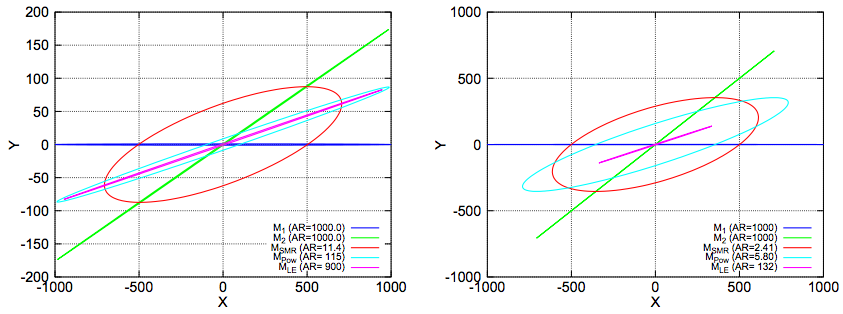
\includegraphics[width=0.95\textwidth]{log_interp.png}
\caption{Log-Euclidean versus Power interpolation
at 1:1000 anisotropy \cite{michal2012anisotropic}}
\label{fig:log_interp}
\end{center}
\end{figure}

\subsection{Implied Metric Field}
\label{sec:ident_metric}

It is often useful to develop an ``implied" metric field
\cite{michal2012anisotropic}.
Given a mesh, the implied metric field is the one which the mesh
currently satisfies.
Since there often does not exist a metric field which is exactly
satisfied, the computed field is an approximation of the field
which is most closely satisfied by the existing mesh.
An implied metric field can be used to maintain a mesh's
initial gradation while responding only to mesh motion.
More importantly, it can be combined with the user's desired
metric field to produce one or more intermediate metric fields
which are more suitable for mesh adaptation
(for example, gradually interpolating from one to the other).

For any simplex element, there exists a single metric tensor
such that all its edges are unit length in metric space, which
implies it is equilateral and has a perfect mean ratio quality
in metric space.
To find this metric, consider that each edge $i$ of the simplex
forms a single scalar constraint:

\begin{equation}
1 = \sqrt{\mathbf{v}_i^T \mathcal{M} \mathbf{v}_i}
\end{equation}

Where $\mathbf{v}_i$ is the real space vector along edge $i$.
Also note that the metric tensor $\mathcal{M}$ has exactly as
many independent scalars as the simplex has edges
($3$ in 2D, $6$ in 3D).
The constraint can be converted into a scalar equation
for the independent variables:

\begin{gather*}
1^2 = \left(\sqrt{\mathbf{v}_i^T \mathcal{M} \mathbf{v}_i}\right)^2 \\
1 = \mathbf{v}_i^T \mathcal{M} \mathbf{v}_i \\
1 = \begin{bmatrix} x_i & y_i & z_i \end{bmatrix}
\begin{bmatrix}
a & d & f \\
d & b & e \\
f & e & c \\
\end{bmatrix}
\begin{bmatrix}
x_i \\
y_i \\
z_i \\
\end{bmatrix} \\
1 = ax_i^2 + by_i^2 + cz_i^2 + 2dx_iy_i + 2ey_iz_i + 2fx_iz_i
\end{gather*}

This leads to a linear system, which following our 3D example
is a $6\times 6$ system:

\begin{equation}
\begin{bmatrix}
x_1^2 & y_1^2 & z_1^2 & 2x_1y_1 & 2y_1z_1 & 2x_1z_1 \\
x_2^2 & y_2^2 & z_2^2 & 2x_2y_2 & 2y_2z_2 & 2x_2z_2 \\
x_3^2 & y_3^2 & z_3^2 & 2x_3y_3 & 2y_3z_3 & 2x_3z_3 \\
x_4^2 & y_4^2 & z_4^2 & 2x_4y_4 & 2y_4z_4 & 2x_4z_4 \\
x_5^2 & y_5^2 & z_5^2 & 2x_5y_5 & 2y_5z_5 & 2x_5z_5 \\
x_6^2 & y_6^2 & z_6^2 & 2x_6y_6 & 2y_6z_6 & 2x_6z_6 \\
\end{bmatrix}
\begin{bmatrix}
a \\ b \\ c \\ d \\ e \\ f
\end{bmatrix}
\begin{bmatrix}
1 \\ 1 \\ 1 \\ 1 \\ 1 \\ 1
\end{bmatrix}
\end{equation}

Where $y_3$ is the $y$ component of the length of edge 3,
and so on.
The matrix and right hand side are formed based on the element
and the linear system is solved via QR decomposition
\cite{trefethen1997numerical}, giving us
the implied metric tensor for an element.
This derivation can be repeated for triangles in 2D, giving
a $3\time 3$ system for the symmetric tensor components.

In order to compute metric tensors at vertices,
We need to conceptually average the implied values obtained
at adjacent elements.
First, we transform the element metric tensors into their
``linear" form, which is one of the forms described
in Section \ref{sec:metric_interp} used for metric interpolation
(for example, Omega\_h uses the matrix logarithm).
Then we take at each vertex the average of these linear
tensors at adjacent elements.
Applying the inverse ``de-linearizing" transformation to the resulting tensor
retries the metric tensor at the vertex.

\subsection{Implied Isotropic Size}
\label{sec:ident_size}

If we are doing isotropic adaptation, we can follow a
similar procedure to that in Section \ref{sec:ident_metric} for metric tensors,
by identifying a desired edge length for each element and averaging
this value to vertices.
This is different from the typical approach of averaging the lengths of edges
adjacent to a vertex, because only considering edges adjacent to the vertex
can produce inaccurate results at corners of even simple meshes, where the
axis-aligned edges are considered but diagonal edges are ignored.
Unlike metric tensors, there rarely exists a single desired length which is
satisfied by all edges of an element.
The approximation we use is the root-mean-square of the element's current
edge lengths ($l_{\text{RMS}}$) defined in Equations \ref{eq:tet_mean_ratio}
and \ref{eq:tri_mean_ratio}.
This is done for consistency with our method of predicting output element counts,
described in Section \ref{sec:elem_count}.

\subsection{Targeting an Element Count}
\label{sec:elem_count}

For users developing a desired metric field, it can be useful
to have the ability to scale their desired metric field such
that the resulting adapted mesh will have a certain desired number
of elements.
This is due to the limited amount of memory on computer systems;
simulations making use of supercomputers will typically approach
the limit of memory when storing their mesh.
Therefore, it is preferable to limit resolution and execute correctly
rather than exceed the memory limit in an attempt to reach high resolution.
Together with re-partitioning onto a larger amount of hardware memory,
metric field scaling should provide better control of parallel adaptive
workflows.

Pain, Umpleby, de Oliveira, and Goddard describe one such method for
predicting the number of elements produced and accordingly adjusting
the metric field \cite{pain2001tetrahedral}.
They begin with the assumption that after mesh adaptation all elements
will have metric volume $\gamma_K$, where $\gamma_K$ is the volume of
a perfectly equilateral tetrahedron with unit edge lengths.
This leads to their volumetric prediction of the new element count
$E_\text{new}$ based on the old elements which are here
numbered from $1$ to $E_\text{old}$:

\begin{equation}
E_{\text{new}} = \frac{\sum_{e=1}^{E_{\text{old}}} \tilde{V}_e}{\gamma_K}
\end{equation}

Where $\tilde{V}_e$ is the volume of element $e$ in metric space,
as we defined in Equation \ref{eq:metric_volume}.
They then seek a scalar $\beta$ such that the scaled size field
$\beta\mathcal{M}$ will produce the desired number of elements
$E_\text{des}$.
They arrive at the following:

\begin{equation}
\beta = \left(\frac{\gamma_K\theta E_{\text{des}}}
{\sum_e^{E_{\text{old}}} \sqrt{\det(\mathcal{M}_e)}V_e}\right)^{2/3}
\end{equation}

Where $\theta$ is a correction factor which they state should
be set to approximately $0.85$.
We claim this correction factor is compensating for the invalidity
of the equilateral-volume assumption.
It is impossible to mesh Euclidean space with equilateral tetrahedra,
and should likewise be difficult in metric space.
We propose using the mean ratios of input elements (in metric space)
as an indication of how far typical element volumes would deviate
from the equilateral volume (recall the interpretation of the
mean ratio from Section \ref{sec:def_quality}).
Instead of summing metric space volumes $\tilde{V}_e$, we sum
the volumes that current elements would have if they were
made equilateral while their root-mean-squared edge length was preserved.
This makes them more comparable to the idealized equilateral
elements being assumed on output:

\begin{equation}
E_{\text{new}} = \frac{\sum_{e=1}^{E_{\text{old}}}
\gamma_K \tilde{l}_{e,\text{RMS}}^3}{\gamma_K}
 = \sum_{e=1}^{E_{\text{old}}} \tilde{l}_{e,\text{RMS}}^3 \\
\end{equation}

This leads to a simpler conclusion: the number of elements that
input element $e$ will become after adaptation is approximately
$\tilde{l}_{e,\text{RMS}}^d$, i.e. its root-mean-squared metric edge length
raised to the power that represents area in 2D or volume in 3D.
See Equations \ref{eq:tet_mean_ratio} and \ref{eq:tri_mean_ratio}
for a definition or root-mean-squared metric length.
This can be used to compute a new metric scaling factor:

\begin{equation} \label{eq:my_metric_scalar}
\beta = \left(\frac{E_{\text{des}}}
{\sum_e^{E_{\text{old}}} \tilde{l}_{e,\text{RMS}}^d}\right)^{2/d}
\end{equation}

Equation \ref{eq:my_metric_scalar} can also be used to compute element weights
to estimate future memory usage for load balancing purposes.

\section{Solution Transfer in a Cavity}

When using mesh adaptation within the context of a simulation,
one needs to maintain the simulation fields defined on the input mesh,
and return similar fields defined on the adapted.
Compared to full re-meshing methods, cavity-based adaptation has the
advantage that field transfer can be localized to cavities, meaning
that fields are only altered where the mesh topology was altered and
that transfer algorithms need only consider this local problem
as opposed to solving complex least-squares fits over the entire meshes.

\subsection{Conserving Integral Quantities}

In order to develop the adaptive Lagrangian hydrodynamics application Alexa
using Omega\_h (see Section \ref{sec:alexa}), we need transfer algorithms
which conserve certain integral quantities.
In particular, our two goals are:
\begin{enumerate}
\item Conserve the mass of each contiguous object in the simulation.
An object may be a fluid body or a solid mass.
Mass is stored as a scalar value at each element.
The algorithm we developed is described in Section \ref{sec:conserve_mass}.
\item Conserve the total momentum of the simulation system.
This is done by using a special algorithm to transfer velocities
(which are stored as vectors at mesh vertices) such that combined
with the above mass transfer they result in momentum conservation.
This algorithm is described in Section \ref{sec:conserve_momentum}.
\end{enumerate}
In both these cases, the additional goal beyond conservation is
the preservation of the variation or distribution of these fields,
as much as possible within the bounds of conservation.
In the context of these algorithms it is useful to define the terms
``donor" and ``target", which indicate the state of the cavity before
and after the mesh is modified, respectively.

\subsubsection{Element-Centered Mass-Like Quantities}
\label{sec:conserve_mass}

The integral conservation requirement for mass can be expressed
in terms of a density field $\rho$, which has donor ($\rho_D$)
and target ($\rho_T$) forms.
Our goal is to find a target density $\rho_T$ such that Equation
\ref{eq:conserve_density} is satisfied,
where $\Omega_D$ is the domain of the donor cavity and
$\Omega_T$ is the domain of the target cavity.

\begin{equation} \label{eq:conserve_density}
\int_{\Omega_T} \rho_T \dd V = \int_{\Omega_D} \rho_D \dd V
\end{equation}

Our discretization of density is such that it has a constant
value in the domain of each element, and is discontinuous between
elements.
We call this space of functions piecewise constants.
The value of density in an element multiplied by the element's
volume is the element mass.
We define two sets of elements: the donor elements $E_D$ and
the target elements $E_T$.
Then discrete conservation is simply an equality of sums,
and the goal is to find target element masses $m_a$.

\begin{equation}
\sum_{a \in E_T} m_a = \sum_{b \in E_D} m_b
\end{equation}

To choose target masses that preserve the density distribution well,
we begin with related work
\cite{jiao2004common,farrell2009conservative} which suggests that
computing the geometric intersections of input and output elements
allows the formulation of good conservative transfer algorithms.
Their method is based on an assumption that donor and target domains
are equal ($\Omega_T=\Omega_D$), and formulating the problem as a
weighted residual of Equation \ref{eq:conserve_density}:

\begin{equation} \label{eq:weighted_residual}
\forall w \in H: \int_{\Omega_T} w \rho_T \dd V = \int_{\Omega_D} w \rho_D \dd V
\end{equation}

Where $H$ is the space of weighting functions, and following
\cite{jiao2004common} we choose $H$ to be the basis function space of the target mesh,
meaning the space of piecewise constant functions on the target mesh.
This just means $H$ can be used to single out each target element,
giving the relationship:

\begin{equation}
\forall a \in E_T: \int_{\Omega_a} \rho_T \dd V
= \int_{\Omega_D \cap \Omega_a} \rho_D \dd V
= \sum_{b \in E_D} \int_{\Omega_b \cap \Omega_a} \rho_D \dd V
\end{equation}

Where $\Omega_a$ is the domain of element $a$, and the intersection of the
domains of two elements $a$ and $b$ is written $\Omega_a \cap \Omega_b$.
Knowing that $\rho_D$ is constant in $\Omega_b$, we get a simple
sum of intersection volumes:

\begin{equation} \label{eq:same_domain_mass}
\forall a \in E_T: \int_{\Omega_a} \rho_T \dd V = m_a
= \sum_{b \in E_D} V(\Omega_b \cap \Omega_a) m_b
\end{equation}

Where $V(\Omega_b \cap \Omega_a)$ is the volume of the intersection of elements $a$ and $b$.
In order to compute this volume, we use the algorithms
proposed by Powell and Abel \cite{powell2015exact} to first compute the polyhedron
which is the intersection of the two element simplices, then compute
its volume.

However, Equation \ref{eq:same_domain_mass} is based on the assumption
that the domains of donor and target cavities are the same, and that
there are not multiple objects requiring separate mass conservation.
In the single object case, adaptation at the boundary of the object may
produce different target and donor domains.
We augment Equation \ref{eq:same_domain_mass} with a correction term
to account for the fact that not all of $\Omega_D$ intersects with $\Omega_T$:

\begin{equation} \label{eq:conserve_mass}
\forall a \in E_T: m_a
= \sum_{b \in E_D} \frac{V(\Omega_b \cap \Omega_a)}
{\sum_{c \in E_T} V(\Omega_b \cap \Omega_c)} m_b
\end{equation}

We can confirm the correctness of Equation \ref{eq:conserve_mass} by
summing all target masses:

\begin{gather*}
\sum_{a \in E_T} m_a
= \sum_{a \in E_T} \sum_{b \in E_D} \frac{V(\Omega_b \cap \Omega_a)}
{\sum_{c \in E_T} V(\Omega_b \cap \Omega_c)} m_b \\
\sum_{a \in E_T} m_a
= \sum_{b \in E_D} \sum_{a \in E_T} \frac{V(\Omega_b \cap \Omega_a)}
{\sum_{c \in E_T} V(\Omega_b \cap \Omega_c)} m_b \\
\sum_{a \in E_T} m_a
= \sum_{b \in E_D} \frac{\sum_{a \in E_T} V(\Omega_b \cap \Omega_a)}
{\sum_{c \in E_T} V(\Omega_b \cap \Omega_c)} m_b \\
\sum_{a \in E_T} m_a
= \sum_{b \in E_D} m_b \\
\end{gather*}

Equation \ref{eq:conserve_mass} can thus conserve mass between
two cavities which may not have the same volume, so long as every
donor element has a non-null intersection with the target cavity
(the sum in the denominator).
This requirement is satisfied for edge collapses (see Figure
\ref{fig:collapse}) and edge swaps (see Figure \ref{fig:swap}),
because in both cases it is true that
all donor elements are adjacent to at least one face of
the relaxed cavity boundary (see Figure \ref{fig:cavity_boundary}),
and each face of the relaxed boundary is also adjacent to
a donor element.
If all donor and target elements have non-zero volume, then
each donor element will overlap with at least one target element
via this boundary face relationship.

Note that in the case of an edge split, every donor element
becomes two target elements of equal volume, so we simply
assign half the donor element mass to each.

\subsubsection{Momentum-Conserving Nodal Velocities}
\label{sec:conserve_momentum}

In the Alexa element formulation, velocity is what we will
call a piecewise linear function.
Its values are stored at vertices, and the value at any point
inside the element is a weighted sum of that element's vertex values,
where the weights are the barycentric coordinates of the point
in the element.

The most important transfer done for piecewise linear fields is that during
refinement, new vertices will receive values via interpolation.
For the refinement operation, this transfer is exact because
it preserves the value of the field at all points in space.
For any other modifications (those that do not create
new vertices) we would typically leave the values at vertices unchanged,
accepting the small perturbations introduced by changes
to the element connectivity.

However, in the case of momentum conservation, we find a need
to modify the vertex velocity values in order to prevent
changing element connectivity from destroying or creating momentum.
The main difficulty here is that the way cavities for edge
collapses and swaps are defined, \emph{there are no vertices on
the interior}.
Recall from Section \ref{sec:cavity} that we require modifications
leave their boundaries unchanged, making it impossible to alter
vertex values without changing the cavity definition.
This leads us to expand our cavity definition for collapses
and swaps, as shown in Figure \ref{fig:buffer_cavity}.
By pushing the boundary outwards by one layer of elements,
we bring the original boundary vertices into the interior
which allows us to modify their values.
In exchange for this, we pay a high price in the complexity
of parallelizing this method, because the selection of independent
sets must now prevent cavities within distance three of
one another from modifying simultaneously (see Section \ref{sec:indset}).
This in turn requires that we increase the amount of ghosting
to three layers during the selection procedure
(see Section \ref{sec:indset_ghost}).

\begin{figure}
\begin{center}
\includegraphics[width=0.6\textwidth]{buffer_cavity.png}
\caption{Cavity with buffer layer and associated notation}
\label{fig:buffer_cavity}
\end{center}
\end{figure}

Because piecewise linear functions are continuous, we cannot
use discontinuity to isolate the cavity as we did in Section
\ref{sec:conserve_mass}.
Instead, we must explicitly require that the new boundary vertices
$\mathcal{N}_F$ remain fixed.
This means the weighted residual technique from Equation
\ref{eq:weighted_residual} is no longer applicable.

The momentum field is the product of the velocity field
and the density field, which in our case is stored as masses
at elements.
The integral of momentum over the domain of an element $e$
can be written as a discrete sum:

\begin{equation} \label{eq:element_momentum}
\mathbf{p}_{e} = m_e \frac1{d+1}\sum_{a \in \mathcal{N}(e)} v_a
\end{equation}

Where $\mathcal{N}(e)$ is the set of vertices of $e$ and
$d$ is the dimensionality of $e$ (assumed to be a simplex),
with vertex velocity values $v_a$.
We begin by leaving the velocity values unchanged between
donor and target, and compute the momentum integrals
over both donor and target cavities.

\begin{gather} \label{eq:sum_over_elems}
\mathbf{p}_T = \sum_{e \in E_T} m_e \frac1{d+1}\sum_{a \in \mathcal{N}(e)} v_a \\
\mathbf{p}_D = \sum_{e \in E_D} m_e \frac1{d+1}\sum_{a \in \mathcal{N}(e)} v_a
\end{gather}

Note that the sum in Equation \ref{eq:sum_over_elems} can be rearranged
to sum over vertices first:

\begin{equation} \label{eq:sum_over_verts}
\mathbf{p}_T = \sum_{a \in \mathcal{N}_T} v_a \frac1{d+1} \sum_{e \in E(a)} m_e
\end{equation}

Where $\mathcal{N}_T$ is the set of vertices in the target cavity and
$E(a)$ is the set of elements adjacent to vertex $a$.
Our momentum conservation method will begin by computing the
momentum loss $(\mathbf{p}_D - \mathbf{p}_T)$, then
we use Equation \ref{eq:sum_over_verts} as the basis for
altering vertex velocities such that each vertex contributes
an equal amount of momentum to the cavity, using these
contributions to correct for momentum loss.
In particular, for a target vertex $a$ the adjusted velocity
$\tilde{v}_a$ is given by Equation \ref{eq:new_velocity}.

\begin{equation} \label{eq:new_velocity}
\forall a \in \mathcal{N}_T:
\tilde{v}_a = v_a +
\frac{{(d+1)}(\mathbf{p}_D - \mathbf{p}_T)}{|\mathcal{N}_T|\sum_{e\in E(a)}m_e}
\end{equation}

In the studies of this method to date we find that the momentum
loss in a cavity is typically a small percentage, i.e.
$(|\mathbf{p}_D - \mathbf{p}T|/\mathbf{p}_D \leq 1\%)$.
For this reason it is less of a concern that we do not take into
account the variation of velocity over space when distributing
these corrections.

The final complication involved in altering these velocities
is that Alexa (and simulation codes in general) apply boundary
conditions involving velocity, meaning they require that vertices
on a subset of the overall mesh boundary have velocity values
which are equal to some user-defined function $v(x,y,z,t)$
over space and time.
This means we should not apply velocity corrections to vertices
with that restriction.
Alexa will identify which boundary surfaces have boundary
conditions applied to them and communicate them Omega\_h.
Omega\_h will then reduce the set
of modified target nodes $\mathcal{N}_T$ in Equation \ref{eq:new_velocity}
accordingly.
If no vertices remain in this set, we disallow that mesh
modification from taking place.
So far this has not been a serious limitation, but care needs to
be taken in areas heavily affected by boundary conditions,
such as the corner of a cube where all three surfaces are
restricted.

Since refinement is exact, it automatically conserves momentum
and does not need to employ the above cavity expansion or velocity
correction.
As discussed in Section \ref{sec:osh_refine}, this is important
because we prefer not to disallow refinement.

\section{Serial Adaptation Performance}

{\bf TODO... }

%%% Local Variables:
%%% mode: latex
%%% TeX-master: t
%%% End:


